\documentclass[conference]{IEEEtran}
\usepackage{amsmath,amssymb,amsfonts,amsthm}
\usepackage{graphicx}
\usepackage{textcomp}
\usepackage{xcolor}
\usepackage{hyperref}
\usepackage{booktabs}
\usepackage{subcaption}

\newtheorem{proposition}{Proposition}

\begin{document}

\title{Action-Space Monitoring as the Foundation Layer\\for VLA Deployment Safety}

\author{\IEEEauthorblockN{Krishnam Gupta}
\IEEEauthorblockA{Independent Research \\
San Francisco, CA \\
kayjee1994@gmail.com}}

\maketitle

\begin{abstract}
Vision-Language-Action (VLA) models predict robot actions end-to-end from vision and language, but the gap between model output and motor command lacks systematic safety infrastructure.
We argue that VLA safety requires defense in depth: multiple independent monitoring layers, each catching failures that others miss.
We contribute \texttt{SafeContract}, a training-free, black-box action-space monitoring toolkit that serves as \emph{Layer~0} of this stack, the always-on physical safety floor beneath higher-level semantic monitors.
Across three architectures (VQ-BeT, Diffusion Policy, ACT) on PushT (2D) and ALOHA (14-DOF bimanual), we show that (1)~different VLA architectures fail in fundamentally different ways, (2)~direction reversal rate is a universal failure predictor (AUROC${=}$0.93, 0.79, 0.91; all $p < 0.001$), while jerk monitoring is predictive only for discrete-token architectures (0.88 vs.\ 0.41), and (3)~split-conformal calibration~\cite{vovk2005} with CUSUM shift detection~\cite{page1954} replaces ad-hoc thresholds with formal coverage guarantees (97.9\% holdout coverage) and bounded false-alarm rates.
SafeContract provides three specific safety properties: bounded actions, bounded velocity, and distribution shift detection.
It does not provide collision avoidance, semantic correctness, or task-level verification, which require complementary higher-layer monitors.
We scope these boundaries precisely.\footnote{Code: \url{https://github.com/krishnam94/vla-edge}}
\end{abstract}

\begin{IEEEkeywords}
VLA, action-space monitoring, defense in depth, failure prediction, conformal prediction, deployment safety
\end{IEEEkeywords}

\section{Introduction}

VLA models~\cite{openvla,smolvla} predict robot actions end-to-end from vision and language.
The dominant deployment pattern today sends these outputs directly to motors with no intermediate safety layer.
OpenVLA's deployment script performs zero bounds checking~\cite{openvla}; pi0 streams actions via WebSocket with no validation~\cite{pi0}; LeRobot's~\cite{lerobot} imperative per-action check is non-composable and easy to omit.
The implicit assumption is that model quality suffices for action safety.
We show this assumption is wrong, and that it is wrong in \emph{architecture-specific} ways.

\textbf{VLA safety is a layered problem.}
No single monitoring approach can address the full failure space of a VLA deployment.
Action-space monitors catch physically unsafe outputs (out-of-bounds, excessive velocity, jerky motion) but cannot detect semantic errors such as reaching for the wrong object.
Internal feature monitors like SAFE~\cite{safe2025} read model uncertainty but require architecture access.
Contrastive verifiers like CoVer-VLA~\cite{cover2026} score vision-language-action alignment but add latency.
VLM-based monitors like Sentinel~\cite{sentinel} reason about task progress but run at 5\,Hz, not 100\,Hz.
The emerging consensus across safe RL, formal methods, and industry practice is defense in depth: independent layers with escalating cost and capability.

Nobody has built the foundation layer.
SafeContract fills this gap: a training-free, black-box toolkit providing always-on physical safety enforcement at $<$0.001\% of VLA inference latency (${\sim}$13\,$\mu$s per call).
It serves as \emph{Layer~0} in a multi-layer monitoring stack (Sec.~\ref{sec:stack}), complementing rather than competing with higher-level monitors.

Our contributions:
\begin{enumerate}
    \item \textbf{VLA architectures fail in fundamentally different ways.} Same-dataset comparison ($n{=}200$, identical seeds and contracts) shows VQ-BeT produces 2.4$\times$ more velocity violations than Diffusion Policy, with qualitatively different failure signatures (Sec.~\ref{sec:closedloop}).
    \item \textbf{No single monitor is universally best.} Direction reversal rate achieves AUROC${=}$0.93 (VQ-BeT) and 0.79 (Diffusion); jerk is predictive only for discrete-token models (0.88 vs.\ 0.41). Monitor selection must be architecture-aware (Sec.~\ref{sec:closedloop}).
    \item \textbf{Formal calibration replaces hand-tuning.} Split-conformal bounds~\cite{vovk2005} achieve 97.9\% holdout coverage with a finite-sample guarantee requiring only exchangeability. CUSUM shift detection~\cite{page1954} provides bounded false-alarm rates that ad-hoc EWMA cannot (Sec.~\ref{sec:calibration}).
\end{enumerate}

\section{Method}

\subsection{Safety Contracts}

A safety contract $C = (\mathbf{l}, \mathbf{u}, v_{\max})$ specifies per-joint action bounds and a velocity limit:
$l_i \leq a_i \leq u_i$ for each joint $i$, and $\|\mathbf{a}_t - \mathbf{a}_{t-1}\|_\infty \leq v_{\max}$.

\textbf{Enforcement order.}
Enforcement proceeds in three phases: (1)~clip to per-joint bounds, (2)~clamp velocity (project each joint's delta onto $[-v_{\max}, v_{\max}]$), (3)~re-clip to bounds.
The final re-clip is necessary because velocity clamping can push actions outside the original bounds.
Any VLA adapter gains monitoring via a one-line \texttt{@safety\_contract} Python decorator on its \texttt{predict()} method.
All violations are logged with timestep, dimension, and magnitude.

\textbf{Composition.}
For hyperrectangular contracts $C_1, C_2$, sequential clipping equals intersection clipping:
$\text{clip}(\text{clip}(\mathbf{a}, C_1), C_2) = \text{clip}(\mathbf{a}, C_1 \cap C_2)$.
Stacking decorators is order-independent for per-joint bounds; velocity composition uses $v_{\max} = \min_i(v_{\max,i})$.

\textbf{Safety properties provided.}
SafeContract enforces three specific properties: (i)~\emph{bounded actions}: every executed action satisfies $l_i \leq a_i \leq u_i$; (ii)~\emph{bounded velocity}: consecutive actions differ by at most $v_{\max}$ per joint; (iii)~\emph{shift detection}: the conformal p-value stream detects when the action distribution departs from calibration data (Sec.~\ref{sec:calibration}).

\textbf{Safety properties NOT provided.}
SafeContract operates only on the action vector.
It cannot detect: (a)~\emph{collision avoidance}, which requires workspace geometry (addressed by CBF methods~\cite{aegis}); (b)~\emph{semantic correctness}, which requires perception and instruction grounding (addressed by contrastive verifiers~\cite{cover2026} and VLM monitors~\cite{sentinel}); or (c)~\emph{task progress}, which requires goal state estimation.
Physically valid actions toward wrong targets are invisible to any action-space monitor.
This is an information-theoretic limitation: semantic correctness is a property of the (action, observation, instruction) triple, not of the action alone.

\subsection{Conformal Anomaly Scoring}
\label{sec:monitoring}

Beyond binary violation detection, each action receives a conformal p-value measuring its anomalousness relative to the calibration distribution.
Given calibration nonconformity scores $\{s_i\}_{i=1}^n$, the p-value of a new action with score $s$ is:
\begin{equation}
p(s) = \frac{|\{i : s_i \ge s\}|}{n+1}
\end{equation}

\begin{proposition}[Coverage guarantee~\cite{vovk2005}]
Under exchangeability of calibration and test data, $P(p \le \alpha) \le \alpha$ for any $\alpha \in (0,1)$.
This is distribution-free, finite-sample, and model-agnostic.
\end{proposition}

The guarantee holds for \emph{any} underlying distribution and \emph{any} sample size $n \ge \lceil 1/\alpha \rceil$.
With $n$ calibration points, coverage lies in $[1{-}\alpha,\; 1{-}\alpha + 1/(n{+}1)]$.
The p-value provides a continuous $[0,1]$ severity measure; departure from uniformity signals distribution shift, testable via Kolmogorov-Smirnov or CUSUM.

\subsection{CUSUM Shift Detection}
\label{sec:cusum}

We use CUSUM~\cite{page1954} for sequential shift detection, which is Lorden-optimal for detecting persistent mean shifts in sequential data.
The statistic accumulates evidence that the anomaly rate exceeds the calibrated rate $\alpha$:
\begin{equation}
S_t = \max(0,\; S_{t-1} + \mathbf{1}[p_t < \alpha] - \alpha)
\end{equation}
An alarm fires when $S_t > h$.
The average run length (ARL) under the null hypothesis satisfies $\text{ARL}_0 = O(e^h / \alpha)$, giving a \emph{formal} false-alarm bound.
EWMA-based alternatives cannot provide such a bound because their ARL depends on the score distribution, which is unknown.

On ALOHA demonstration data with conformal p-values feeding the CUSUM: in-distribution actions produce zero alarms; adding $\sigma{=}0.1$ Gaussian noise triggers detection within 7 steps (threshold $h{=}3$).

Additionally, \textbf{clip magnitude} $m_i = |a_i^{\text{raw}} - a_i^{\text{clipped}}|$ provides a free, per-joint signal that remains informative when violation counts saturate.

\subsection{Conformal Calibration}
\label{sec:calibration}

Hand-tuned thresholds are unreliable: a common choice of $v_{\max}{=}0.05$ clips a significant fraction of \emph{expert} actions on the ALOHA dataset.
We replace hand-tuning with split-conformal prediction~\cite{vovk2005}.
Demonstration episodes are split 80/20; nonconformity scores $s_i = \max_j |a_{ij} - \hat{\mu}_j| / \hat{\sigma}_j$ are computed on the calibration set; the $\lceil(1{-}\alpha)(1 + 1/n)\rceil$-th quantile yields bounds with a finite-sample coverage guarantee.

At $\alpha{=}0.05$, conformal bounds are 25\% tighter than the 4$\sigma$ heuristic while achieving 97.9\% holdout coverage (99.1\% minimum per dimension).
The coverage guarantee holds under exchangeability with calibration data; during deployment, coverage degrades under distribution shift.
CUSUM (Sec.~\ref{sec:cusum}) detects when this occurs; adaptive conformal inference~\cite{gibbs2021} would maintain coverage online by dynamically adjusting $\alpha_t$.

Velocity limits are set per-joint at the 99th percentile of consecutive action deltas from the calibration set (an empirical heuristic, not a conformal guarantee).

\subsection{Architecture-Specific Monitors}
\label{sec:health}

Bounds and velocity checks miss architecture-specific failure modes.
We add targeted monitors:

\noindent\textbf{Stall detection.}
Diffusion policies' primary failure mode is policy freeze: valid-looking micro-movements where the robot barely moves~\cite{safe2025}.
StallDetector flags when $\|\mathbf{a}_t - \mathbf{a}_{t-1}\|_2 < \tau$ for $w$ consecutive steps.

\noindent\textbf{Jerk monitoring.}
The third derivative of the action trajectory detects denoising artifacts in diffusion policies and chunk boundary discontinuities in action-chunked policies~\cite{acg2025}.

\noindent\textbf{Direction reversal rate.}
For each joint $j$, a reversal occurs when $\text{sign}(a_{t,j} - a_{t-1,j}) \neq \text{sign}(a_{t-1,j} - a_{t-2,j})$.
The episode reversal rate averages over all (timestep, joint) pairs.
High reversal rates indicate oscillatory or indecisive behavior.

\noindent\textbf{Gripper oscillation.}
Rapid open/close cycling (more than $k$ flips in $w$ steps) signals grasp indecision in bimanual manipulation.

\section{The Monitoring Stack}
\label{sec:stack}

SafeContract occupies Layer~0 in a multi-layer defense-in-depth architecture for VLA deployment.
Each layer operates independently and catches failures that other layers miss:

\smallskip
\noindent\textbf{Layer~0: Action-Space Enforcement} ($<$1\,ms). SafeContract, AEGIS CBF~\cite{aegis}. Bounds, velocity, jerk. Always-on physical safety floor. Cannot detect semantic failures.

\noindent\textbf{Layer~1: Internal Feature Monitoring} (${\sim}$1\,ms). SAFE~\cite{safe2025}, FIPER~\cite{fiper2025}. Reads model uncertainty from VLA internals. Requires architecture access.

\noindent\textbf{Layer~2: Contrastive Verification} (${\sim}$8\,ms). CoVer-VLA~\cite{cover2026}. Scores vision-language-action alignment. Catches wrong-object selection.

\noindent\textbf{Layer~3: VLM Semantic Monitoring} (${\sim}$200\,ms). Sentinel~\cite{sentinel}. Full semantic reasoning about task progress. Catches compositional failures but too slow for per-action use.
\smallskip

This layering mirrors established safety-critical practice: aviation stacks stall warning, GPWS, and TCAS as independent layers; automotive ASIL decomposes across redundant channels; ISO~10218 separates workspace monitoring from controller limits.
The EU AI Act (Article~9) will mandate continuous monitoring for high-risk AI systems by June~2027~\cite{euaiact}, creating a regulatory requirement for exactly this kind of layered runtime monitoring infrastructure.

SafeContract's value in this stack is threefold: (i)~it is the only layer requiring \emph{zero} model access, auxiliary training, or additional sensors; (ii)~it runs at ${\sim}$13\,$\mu$s, three orders of magnitude faster than any other layer; (iii)~it provides \emph{enforcement} (clipping), not just detection.

\section{Related Work}

\textbf{Training-time safety.}
SafeVLA~\cite{safevla} and RobustVLA~\cite{robustvla} improve safety via retraining or fine-tuning.
These are complementary to runtime monitoring: training-time safety reduces violation frequency but cannot handle distribution shift, hardware degradation, or the erosion of safety alignment under LoRA fine-tuning~\cite{safevla}.

\textbf{Inference-time safety.}
AEGIS~\cite{aegis} solves a CBF-QP per step (0.36\,ms, requiring dynamics models); SafeDiffuser~\cite{safediffuser} and CoDiG~\cite{codig} embed barriers in diffusion (architecture-specific); SafeDec~\cite{safedec} constrains decoding; Safety Chip~\cite{safetychip} uses LTL monitors; ATACOM~\cite{atacom} projects onto constraint manifolds.
All require dynamics models, architecture access, or retraining.

\textbf{Failure detection.}
SAFE~\cite{safe2025} trains a failure detector on VLA internal features; FIPER~\cite{fiper2025} trains an RND network for failure prediction; Sentinel~\cite{sentinel} monitors temporal consistency and task progress.
These require training auxiliary models and operate at Layers~1--3 of the monitoring stack.
SafeContract is the only approach at Layer~0: training-free, black-box, and providing enforcement rather than detection alone.

\textbf{Conformal prediction for safety.}
Recent work validates conformal prediction for robot safety~\cite{safe2025,feldman2025}.
Kim et al.~\cite{kim2026guardrails} argue that modular guardrails are necessary for foundation-model robots.
We use split-conformal bounds~\cite{vovk2005} for action-space coverage and conformal p-values with CUSUM~\cite{page1954} for shift detection, providing a concrete, calibrated implementation of this modular guardrail argument.

\section{Experiments}

Platform: Apple M3, CPU, Python 3.12. Full monitoring overhead: $<$0.001\% of typical VLA inference time (${\sim}$13\,$\mu$s per call).

\subsection{VLAs Produce Unsafe Actions (EXP-A)}
\label{sec:exp_a}

We run SmolVLA on 100 consecutive LIBERO observations with SafeContract monitoring.
After correct MEAN\_STD unnormalization, bounds violations drop from 86\% to 0\%: every bounds violation was a normalization artifact, detectable by monitoring.
The robust finding is velocity: at $v_{\max}{=}0.1$ rad/step, \textbf{98\%} of SmolVLA steps violate on at least one joint versus \textbf{16\%} of expert steps, a \textbf{6$\times$ gap} that persists regardless of normalization.

\begin{figure}[t]
    \centering
    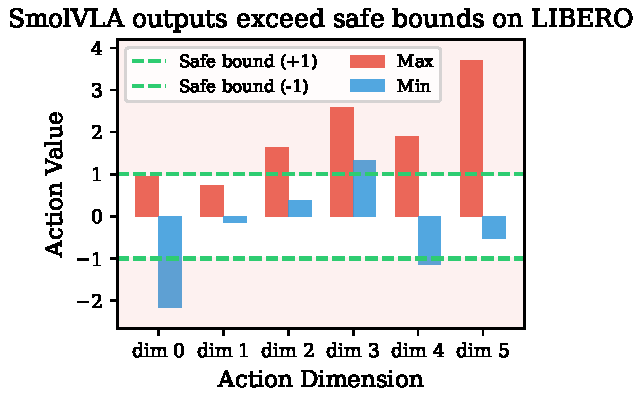
\includegraphics[width=\columnwidth]{figures/fig1_action_ranges.pdf}
    \caption{SmolVLA action ranges on 100 LIBERO observations. Most dimensions exceed the $[-1, 1]$ bounds (green dashes), reflecting normalization mismatch between SO-100 training data and LIBERO's action space.}
    \label{fig:action_ranges}
\end{figure}

\subsection{Same-Dataset Cross-Architecture (EXP-CL)}
\label{sec:closedloop}

We evaluate two architectures on the \emph{same} PushT dataset with the same seeds (0--199), contract (bounds $[0, 512]$, $v_{\max}{=}30$\,px/step), and success criterion (coverage ${\ge}0.95$).
This controls for task and environment, isolating architecture effects.

\textbf{Diffusion Policy}~\cite{diffusionpolicy} (262M params, DDPM, $n{=}200$ per condition).
Without SafeContract: 58\% success (116/200, CI$_{95}$: [0.51, 0.65]).
With SafeContract: 57\% success (114/200, CI$_{95}$: [0.50, 0.64]).
Fisher's $p = 0.92$. SafeContract caught 772 violations with no task degradation.

\textbf{VQ-BeT}~\cite{vqbet} (37.5M params, VQ-VAE + Behavior Transformer, $n{=}200$).
Without SafeContract: 56.5\% success (113/200, CI$_{95}$: [0.50, 0.63]).
With SafeContract: 54.5\% success (109/200, CI$_{95}$: [0.48, 0.61]).
Fisher's $p = 0.76$. SafeContract caught 1{,}847 velocity violations with no significant degradation.

The architecture contrast: on the same task, VQ-BeT produces 2.4$\times$ more violations than Diffusion (1{,}847 vs.\ 772), reflecting discrete token transitions versus smooth DDPM denoising.

\textbf{Note on success rates.}
Our Diffusion Policy achieves 58\% vs.\ the published 87.4\%. This gap reflects evaluation protocol: we use the LeRobot pretrained checkpoint with 300-step episodes and strict coverage $\ge 0.95$, while Chi et al.\ use 1{,}000-step episodes with relaxed thresholds.
VQ-BeT achieves 56.5\% (published: 57\%), confirming correct reproduction.
Both use identical evaluation conditions, making the cross-architecture comparison valid.

\textbf{ACT on ALOHA}~\cite{act} (51.6M params, 14-DOF bimanual, $n{=}50$ per condition).
Without SafeContract: 62\% success (31/50, CI$_{95}$: [0.48, 0.74]).
With SafeContract: 56\% success (28/50, CI$_{95}$: [0.42, 0.69]).
Fisher's $p = 0.68$. SafeContract caught 4{,}758 velocity violations with no significant degradation.

Across all three architectures, SafeContract monitors and enforces without statistically significant task degradation ($p{=}0.92$, $p{=}0.76$, $p{=}0.68$).

\begin{figure}[t]
    \centering
    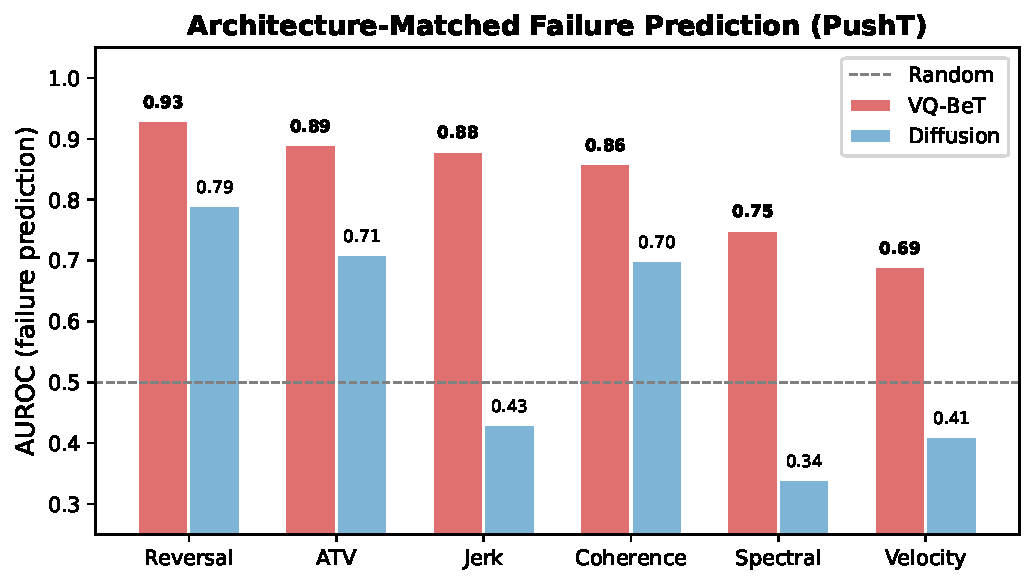
\includegraphics[width=\columnwidth]{figures/fig_auroc_comparison.pdf}
    \caption{Architecture-matched failure prediction (PushT, $n{=}100$). Reversal rate predicts failure with AUROC${=}$0.93 (VQ-BeT) and 0.79 (Diffusion). Jerk monitoring is predictive only for discrete-token architectures. No single monitor is universally best.}
    \label{fig:auroc}
\end{figure}

\begin{figure}[t]
    \centering
    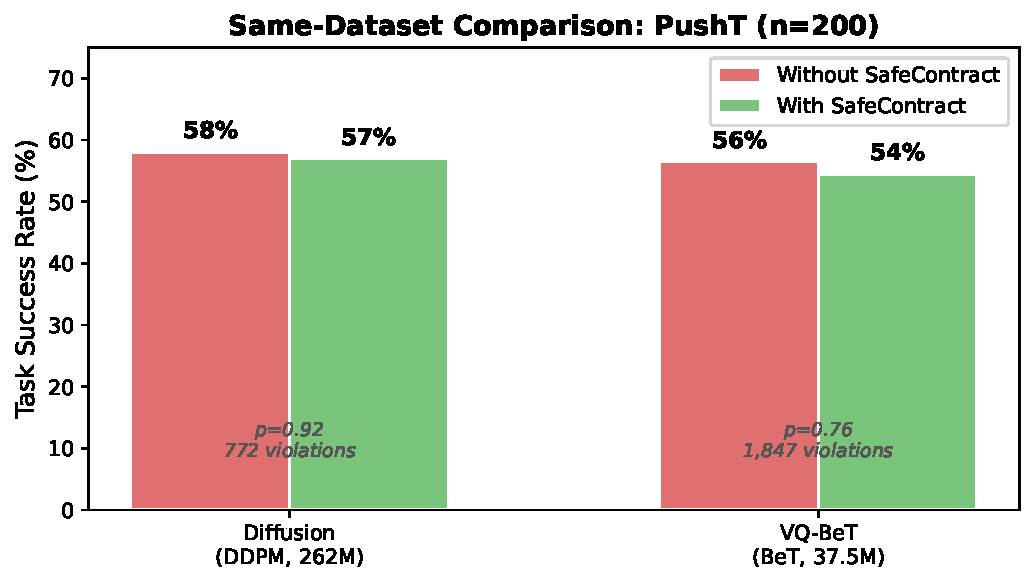
\includegraphics[width=\columnwidth]{figures/fig_pusht_comparison.pdf}
    \caption{Same-dataset closed-loop comparison on PushT ($n{=}200$ per condition). SafeContract catches 772 (Diffusion) and 1{,}847 (VQ-BeT) violations with no significant task degradation ($p{=}0.92$ and $p{=}0.76$).}
    \label{fig:closedloop}
\end{figure}

\textbf{Failure prediction with bootstrap confidence intervals.}
Table~\ref{tab:crossarch} reports AUROCs for five monitors across three architectures, with bootstrap 95\% CIs (2{,}000 resamples).
Direction reversal rate predicts task failure with AUROC${=}$0.93 [0.88, 0.97] on VQ-BeT, 0.79 [0.69, 0.88] on Diffusion, and 0.91 [0.79, 0.99] on ACT/ALOHA ($p < 0.001$ all three), confirming it as a universal failure predictor across architectures and action dimensions (2D and 14-DOF).
Jerk monitoring is strongly predictive for VQ-BeT (0.88 [0.81, 0.94]), moderately for ACT (0.69 [0.54, 0.84]), and not for Diffusion (0.41 [0.30, 0.54]), a gradient consistent with the discrete-to-continuous architecture spectrum.
Velocity violations are non-predictive across all three (0.41--0.69), confirming that monitor selection matters more than the monitoring paradigm.

\begin{table*}[t]
\centering
\caption{Cross-architecture comparison with failure prediction AUROCs and bootstrap 95\% CIs (2{,}000 resamples). PushT: $n{=}200$ per condition (same seeds/contract), AUROCs computed on $n{=}100$. ALOHA: $n{=}50$ per condition, AUROCs on $n{=}50$. Bold indicates AUROC $\ge 0.80$.}
\label{tab:crossarch}
\small
\begin{tabular}{lccc}
\toprule
 & \textbf{Diffusion (PushT)} & \textbf{VQ-BeT (PushT)} & \textbf{ACT (ALOHA 14-DOF)} \\
\midrule
Family & Continuous & Discrete & Continuous \\
Params & 262M & 37.5M & 51.6M \\
Success (no / with contract) & 58\% / 57\% & 56.5\% / 54.5\% & 62\% / 56\% \\
Fisher's $p$ & 0.92 & 0.76 & 0.68 \\
Violations & 772 & \textbf{1{,}847} & 4{,}758 \\
\midrule
AUROC: reversal rate & 0.79\,[0.69, 0.88] & \textbf{0.93}\,[0.88, 0.97] & \textbf{0.91}\,[0.79, 0.99] \\
AUROC: jerk & 0.41\,[0.30, 0.54] & \textbf{0.88}\,[0.81, 0.94] & 0.69\,[0.54, 0.84] \\
AUROC: momentum coherence & 0.70\,[0.58, 0.80] & \textbf{0.86}\,[0.78, 0.93] & 0.71\,[0.57, 0.85] \\
AUROC: spectral energy & 0.34\,[0.23, 0.46] & 0.75\,[0.65, 0.84] & 0.74\,[0.59, 0.87] \\
AUROC: velocity & 0.41\,[0.30, 0.53] & 0.69\,[0.58, 0.79] & 0.52\,[0.35, 0.68] \\
\bottomrule
\end{tabular}
\end{table*}

\section{Discussion}

\textbf{Architecture-specific failure signatures.}
The central finding is that different VLA architectures fail in fundamentally different ways.
Across three architectures and two tasks, direction reversal rate is the most universal predictor (AUROC: 0.93, 0.79, 0.91), while jerk follows a discrete-to-continuous gradient (0.88, 0.41, 0.69).
VLA architectures partition into two families: a \emph{discrete family} (autoregressive, VQ-VAE) where jerk and reversal rate are strongly predictive, and a \emph{continuous family} (diffusion, flow matching, action chunking) where momentum coherence and reversal rate matter more.
ACT on ALOHA (14-DOF) confirms this: as a continuous-family model with chunk boundary effects, its jerk AUROC (0.69) falls between VQ-BeT (0.88) and Diffusion (0.41).

\textbf{Practical implications.}
Practitioners must select monitors based on their VLA architecture.
For discrete-token models (VQ-BeT, OpenVLA), jerk and reversal rate are the strongest predictors.
For smooth denoisers (Diffusion, flow matching), momentum coherence and reversal rate are more reliable.
\texttt{SafetyGuard}, SafeContract's top-level API, integrates all monitors in a single callable calibrated from demonstration data:

{\small
\begin{verbatim}
guard = SafetyGuard.from_demos(demo_actions)
@guard.wrap  # clip + stall + jerk + p-value
def predict(self, obs): ...
\end{verbatim}
}
\vspace{-2mm}
\noindent No hand-tuning, no model internals, no retraining.

\textbf{The hybrid architecture limitation.}
Emerging hybrid VLAs (e.g., DiffusionVLA, HybridVLA, GR00T~N1) split the pipeline into an autoregressive backbone for reasoning and a diffusion head for action generation.
The diffusion head produces smooth, bounded, kinematically valid actions by construction.
When the reasoning component is wrong, the action head generates physically valid trajectories toward wrong targets.
These failures pass every action-space monitor, including SafeContract.
This is the fundamental boundary of Layer~0 monitoring: it enforces physical safety but is provably blind to semantic correctness.
For hybrid architectures, Layers~1--3 (internal features, contrastive verification, VLM reasoning) are essential complements.

\textbf{Conformal coverage in practice.}
The 97.9\% conformal coverage guarantee holds under exchangeability with calibration data.
In deployment, the exchangeability assumption fails progressively as the robot encounters novel situations.
CUSUM detects when this occurs (Sec.~\ref{sec:cusum}): the violation rate against conformal bounds serves as a sufficient statistic for distribution shift, because an observed rate significantly exceeding $\alpha$ rejects the exchangeability null hypothesis.
Adaptive conformal inference~\cite{gibbs2021} would maintain coverage online by adjusting $\alpha_t \leftarrow \alpha_t + \gamma(\alpha - \text{err}_t)$.

\textbf{Limitations.}
(1)~All experiments in simulation; real-robot action distributions may differ.
(2)~Three of eleven known VLA architecture types tested; autoregressive (OpenVLA) and flow matching (pi0) remain untested.
(3)~The conformal coverage guarantee is marginal (averaged over test points), not conditional on specific observations.
(4)~Bootstrap CIs for ALOHA AUROCs are wide ($n{=}50$); larger-scale evaluation would tighten them.

\textbf{Future work.}
Extensions to autoregressive and flow-matching architectures;
adaptive conformal inference for online recalibration;
real-robot validation;
and formal integration with Layers~1--3 to build a complete monitoring stack.

\begin{thebibliography}{25}
\bibitem{openvla} Kim, M.J. et al., ``OpenVLA: An Open-Source Vision-Language-Action Model,'' CoRL 2024, arXiv:2406.09246.
\bibitem{smolvla} Shukor, M. et al., ``SmolVLA: A Vision-Language-Action Model for Affordable and Efficient Robotics,'' arXiv:2506.01844, 2025.
\bibitem{lerobot} Cadene, R. et al., ``LeRobot: State-of-the-art Machine Learning for Real-World Robotics in PyTorch,'' 2024, \url{https://github.com/huggingface/lerobot}.
\bibitem{pi0} Black, K. et al., ``$\pi_0$: A Vision-Language-Action Flow Model for General Robot Control,'' arXiv:2410.24164, 2024.
\bibitem{safevla} Zhang, B. et al., ``SafeVLA: Towards Safety Alignment of Vision-Language-Action Model via Constrained Learning,'' NeurIPS 2025, arXiv:2503.03480.
\bibitem{aegis} Hu, S. et al., ``VLSA: Vision-Language-Action Models with Plug-and-Play Safety Constraint Layer,'' arXiv:2512.11891, 2025.
\bibitem{safedec} Kapoor, P. et al., ``Constrained Decoding for Robotics Foundation Models,'' arXiv:2509.01728, 2025.
\bibitem{robustvla} Guo, J. et al., ``On Robustness of VLA Models against Multi-Modal Perturbations,'' ICLR 2026.
\bibitem{safetychip} Yang, Z. et al., ``Plug in the Safety Chip: Enforcing Constraints for LLM-driven Robot Agents,'' ICRA 2024.
\bibitem{safediffuser} Xiao, W. et al., ``SafeDiffuser: Safe Planning with Diffusion Probabilistic Models,'' ICLR 2025.
\bibitem{codig} Ma, H. et al., ``CoDiG: Constraint-Aware Diffusion Guidance for Robotics,'' CoRL 2025.
\bibitem{atacom} Tolle, M. et al., ``Towards Safe Robot Foundation Models Using Inductive Biases,'' arXiv:2505.10219, 2025.
\bibitem{sentinel} Agia, C. et al., ``Unpacking Failure Modes of Generative Policies: Runtime Monitoring of Consistency and Progress,'' CoRL 2024, arXiv:2410.04640.
\bibitem{vovk2005} Vovk, V. et al., ``Algorithmic Learning in a Random World,'' Springer, 2005.
\bibitem{page1954} Page, E.S., ``Continuous Inspection Schemes,'' Biometrika 41(1/2):100--115, 1954.
\bibitem{safe2025} Gu, Q. et al., ``SAFE: Multitask Failure Detection for Vision-Language-Action Models,'' NeurIPS 2025, arXiv:2506.09937.
\bibitem{fiper2025} Romer, R. et al., ``Failure Prediction at Runtime for Generative Robot Policies,'' NeurIPS 2025, arXiv:2510.09459.
\bibitem{feldman2025} Feldman, A.O. et al., ``Conformal Safety Monitoring for Flight Testing,'' arXiv:2511.20811, 2025.
\bibitem{gibbs2021} Gibbs, I. and Candes, E., ``Adaptive Conformal Inference Under Distribution Shift,'' NeurIPS 2021, arXiv:2106.00170.
\bibitem{acg2025} Park, M. et al., ``ACG: Action Coherence Guidance for Flow-based VLA Models,'' arXiv:2510.22201, 2025.
\bibitem{kim2026guardrails} Kim, J. et al., ``Modular Safety Guardrails Are Necessary for Foundation-Model-Enabled Robots in the Real World,'' arXiv:2602.04056, 2026.
\bibitem{diffusionpolicy} Chi, C. et al., ``Diffusion Policy: Visuomotor Policy Learning via Action Diffusion,'' RSS 2023, arXiv:2303.04137.
\bibitem{vqbet} Lee, S. et al., ``Behavior Generation with Latent Actions,'' ICML 2024, arXiv:2403.03181.
\bibitem{act} Zhao, T.Z. et al., ``Learning Fine-Grained Bimanual Manipulation with Low-Cost Hardware,'' RSS 2023, arXiv:2304.13705.
\bibitem{cover2026} Tang, W. et al., ``CoVer-VLA: Contrastive Verification for Vision-Language-Action Models,'' arXiv:2602.12281, 2026.
\bibitem{euaiact} European Commission, ``Regulation (EU) 2024/1689 (AI Act),'' Official Journal of the European Union, 2024, Article 9: Risk Management System.
\end{thebibliography}

\end{document}
